%
%  $Description: Author guidelines and sample document in LaTeX 2.09$
%
%  $Author: ienne $
%  $Date: 1995/09/15 15:20:59 $
%  $Revision: 1.4 $
%

\documentclass[times, 10pt,twocolumn]{article}
\usepackage{latex8}
\usepackage{times}
\usepackage{balance}
\usepackage{epsfig}
\usepackage{graphicx}
\usepackage{url}
%\usepackage{wrapfig}

%\documentstyle[times,art10,twocolumn,latex8]{article}

%-------------------------------------------------------------------------
% take the % away on next line to produce the final camera-ready version
\pagestyle{empty}

%-------------------------------------------------------------------------
\begin{document}

\title{Beyond The Kiss-Cam: Measuring The Fan Using Computer Vision-based Analytics}

\author{George Williams  \hspace{0.1in} Christoph Bregler \hspace{0.1in} Ian Spiro \hspace{0.1in} \\
\emph{Dept. of Computer Science, Courant Institute, New York University}\\
\emph{george,chris,ian@movement.nyu.edu}\\
% For a paper whose authors are all at the same institution,
% omit the following lines up until the closing ``}''.
% Additional authors and addresses can be added with ``\and'',
% just like the second author.
%\and
%Second Author\\
%Institution2\\
%First line of institution2 address\\ Second line of institution2 address\\
%SecondAuthor@institution2.com\\
}


\maketitle

\thispagestyle{empty}

\begin{abstract}
What are fans really doing at the game?  When are they watching the action on the field/court, and when are they buried in their phone or tablet?  Which ads do they notice on the JumboTron, and which ones do they ignore?  Who’s joining in the “wave” and who’s not?  Are they having fun?

If you are a club trying to retain seat-buying fans, fill empty chairs, or effectively use an advertising budget, then these are important questions to answer. Video surviellance tools can help, but sifting through crowd footage does not scale.

In this paper, we describe a computer vision-based software method that goes beyond just capturing videos.  We propose a machine learning-based framework that can automatically recognize certain kinds of fan activity.  Our technique is based on convolutional neural networks and it leverages crowd-sourcing to inexpensively and quickly build a training database.

We conducted experiments on crowd footage of a college basketball game and describe our results.  Importantly, we show how its possible to preserve the anonymity of the fans.

\end{abstract}

%-------------------------------------------------------------------------
\Section{Introduction}

In 2012, TicketMaster reported that 26\% of available stadium seat tickets went unsold, representing an estimated loss of 100 millions dollars for the year \cite{ticketmaster}.  To better understand their fans and customers, many clubs and the major ticketing agencies have turned to analytics to help bridge this revenue gap.  So-called ``fanalytics'' attempts to extract meaningful information from a mountain of information- from ticket purchase history to the opinions and comments expressed by fans on blogs and social media  \cite{fanalytics}.  Yet, comparatively less work has been done to learn precisely what fans enjoy or don't like about attending a live event.   

Customer interviews, surveys, and questionnaires might be useful but they are limited due to their ad-hoc and voluntary nature.  Moreover, it may not be clear what to ask fans about their experience.  They may not remember why exactly they weren't watching a particular ad or why they weren't engaged in the game action at a specific point in time.  Clearly, the direct observation of fans would be an invaluable tool.  Capturing fans on video is a start, but how can such observation scale to large stadium crowds?  How do you ensure fan privacy?     

We explore a software approach to overcome these obstacles, using a method we call 'site-specific learning.'  The idea is conceptually simple.  We record video of the fans at a game.  Then, we use a portion of the crowd video footage to train a convolutional neural network.  When trained properly, this neural network has the ability to recognize and detect chosen types of fan activity, in all of the footage.  

\begin{figure}[bt]
\centering
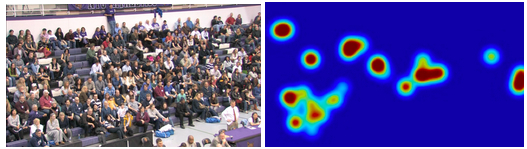
\includegraphics[width=0.96\columnwidth]{fanheat}
\caption{\label{fig_fanheat} \small A heat map which indicates the clapping fans in a frame of video, automatically detected by the neural network. }
\end{figure}

Figure \ref{fig_fanheat} demonstrates a result.  The heatmap, on the right, shows locations of the fans, on the left, performing the same activity, in this case, clapping. 

%-------------------------------------------------------------------------
\section{Related Work}
\label{sec_related}

``Fanalytics'' covers a broad range of topics in fan-based analytics as it pertains to driving revenue, including ticketing analysis and dynamic pricing models \cite{fanalytics} \cite{ticketmaster} \cite{ticketmaster2} \cite{ticketinganalytics} \cite{ticketinganalytics2}.

From a computer vision standpoint, our work most closely fits into the categories of ``crowd image analysis'' or ``surveillance tracking'', for which there are dedicated workshops and conferences \cite{pets} \cite{msvalc}.  In particular, we were inspired by the following papers \cite{trackingunstructured} \cite{trackingsmallgroups} in this domain.

Since our method detects individual fans and isolates their activity, we also draw upon a body of research in activity recognition that spans several decades and many conferences \cite{modelbasedimage} \cite{modelbasedvision} \cite{humanmotionanalysis} \cite{threedeemodel} \cite{modelrec} \cite{modelbasedtracking} \cite{trackingpeople} \cite{modelbasedest} \cite{articbody} \cite{stochastic}.

This paper does does not address how to interpret fan behavior, once its isolated from the original footage.  An assessment of fan engagement may involve, for example, more than detecting obvious forms of expressive positive sentiment like clapping or cheering.  Interpreting human gesture is an active area of research and involves a multidisciplinary approach from diverse areas such as human anatomy and psychology.  For the interested researcher we recommend the following reading as a starting point \cite{laban}.

Our technique leverages the Amazon Mechanical Turk service for labeling the fan's activity in captured video.  More information about this service can be found here \cite{amazon}.  

%-------------------------------------------------------------------------
\section{Approach}

The basic steps involved in our approach are summarized as follows:

\begin{itemize}
\item 1. Collect lots of video footage of the crowd at a game and venue.
\item 2. Perform face detection on the video.
\item 3. Isolate the body around each face detected and extrapolate short video clips of the fan ( we call these ``fidgets'' ).
\item 4. Randomly select a subset of fidgets and manually identify the fan’s behavior in each ( we call this process ``labeling'' ).
\item 5. From the set of labels, choose an activity ( like, clapping ).
\item 6. Create a training database comprised of the labeled fidgets.
\item 7. Train a neural network using the training database, and monitor its progress using a validation dataset ( a portion of the original training set aside for this purpose ).
\item 8.  Use the trained neural network to detect the activity of interest in all of the fidgets for all of the videos.
\item 9.  Repeat steps 4-8 for another activity of interest.
\end{itemize}

The following sections explore the stages of this pipeline in further detail.  Mainly, we demonstrate how we created a clapping-fan detector using video footage of the crowd watching a college basketball game.  The method generalizes to other types of fan activity.

\subsection{Data Collection: Game Day}
\label{sec_GameDay}

We set up 4 HD cameras at a college basketball game and positioned them above the audience at balcony level.  We aimed 3 cameras at the most populated areas of the stands.  The camera views did not overlap.  We manually adjusted the zoom in order to capture as many fans as possible in each view, but not so far zoomed-out that each face spanned no less than around 20 pixels ( the software-based face detector has difficulty detecting faces less than 20 pixels.)  We aimed the final camera at the basketball game and adjusted the zoom to capture the action at both ends of the court, including the scoreboard which hovered above the center of the court.  Figure \ref{fig_cams} shows 2 of the camera views.

\begin{figure}[bt]
\centering
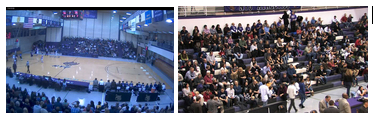
\includegraphics[width=0.96\columnwidth]{cams}
\caption{\label{fig_cams} \small Two of the camera views of crowd footage. }
\end{figure}

We recorded the entirety of two basketball games, a women’'s college game and a men’'s college game.

\subsection{Face Detection}
\label{sec_facedet}

The first stage in our data processing pipeline is software-based face detection.  We used an off-the-shelf face detector from PittPatt.com, a company which was acquired by Google in 2012 \cite{pittpattgoogle}.  Since we use face detection to detect fans, it was important to capture as many faces as possible.  Highly accurate face detection can be time-consuming, so instead of each frame we performed face detection on every 50th frame.  We felt we could justify this optimization because, over the course of a game, a fan is not likely to change their position appreciably, especially over a 50 frame period.  
\subsection{Fidgets}
\label{sec_fidgets}

For each face detected, we extracted a region of interest larger than the face itself.  This was an attempt to capture the person'’s entire body, not just their face.  We experimented with several parameters.  We found that by increasing the height of the face detection bounding box by a factor of 4 and the length by a factor of 3, we could capture the fan not only sitting but also standing as well.  We applied this region of interest to the following 39 frames that followed the face detection frame, resulting in a small 40 frame video clip of the fan that we call a ``fidget.''

The fidget may or may not contain anything interesting, and in general, most fidgets do not.  Also, the length of 40 frames ( a little over 1 second for our 30 FPS video ) might seem short.  But, as it turns out, a 40-frame fidget is enough to capture a myriad of distinct fan activities including clapping, talking, cheering, eating, using a cell phone, etc.  It was important to keep the number of frames as small as possible as not to overload inputs of the neural network later on.  Figure \ref{fig_fidget} shows the first five frames of an example fidget of a fan clapping:

\begin{figure}[bt]
\centering
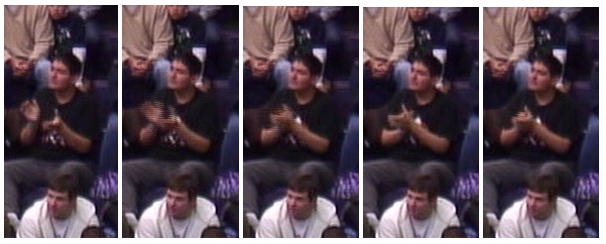
\includegraphics[width=0.96\columnwidth]{fidget}
\caption{\label{fig_fidget} \small The first five frames of a sample fidget. }
\end{figure}

\subsection{Machine Learning}
\label{sec_machinelearning}

Our approach is based on machine learning, and specifically, a class of algorithms called convolutional neural networks.  Convolutional Neural Networks (a corner stone of Deep Learning \cite{deeplearning}) are not new, but recent advances in compute power make training and using these learning algorithms more practical than ever.

A treatment of the state-of-the-art in neural networks and machine learning is beyond the scope of this paper, but they all have one thing in common - they all require a learning phase in which the algorithm is trained on lots of examples.  

\subsection{Building A Training Database}
\label{sec_traindb}

To build a training database for our neural network, we used a small portion of the video we collected at the event.  We randomly sampled a small subset of the fidgets extracted in a previous step and then identified the fan's activity, such as clapping, cheering, talking, etc.  Labeling on this scale can be time consuming, so, to save on time, we crowd-sourced the job to hundreds of workers via Amazon Mechanical Turk.  Figure \ref{fig_turk} shows the task we presented to the workers.  

\begin{figure}[bt]
\centering
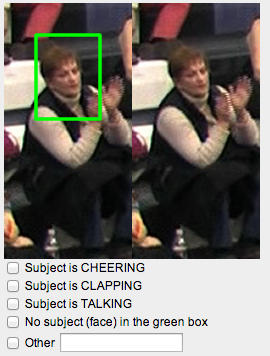
\includegraphics[width=0.96\columnwidth]{turk}
\caption{\label{fig_turk} \small The labeling task we presented the Turkers. }
\end{figure}

To ensure label accuracy, we presented each fidget to three different Turkers.  If a majority answered the same way, then we accepted the Turks’ label for this fidget.  We paid two cents per task.

\subsection{Training The Neural Network}
\label{sec_train}

This section summarizes how we trained the convolutional neural network for this event, so readers not familiar with neural networks may want to skip it.  For a tutorial on convolutional neural networks architecture, please see \cite{deeplearning}.

The training database we presented to this neural network was comprised of a total of about 1840 Turk-labeled fidgets, 940 were ``positive'' training samples of fan’s clapping and 900 were ``negative'' training samples, comprised of fans that were either cheering or talking but not clapping.  20\% of each set were set aside as a validation set, which was used during the training phase to guage its progress.

Before training, the neural network weights were randomized.  During each training iteration, or epoch, a new batch of 8 fidgets were randomly sampled from the training database,  4 from the positive set, and 4 from the negative set.  

The processing performed in each epoch is summarized as follows:
\begin{itemize}
\item each fidget in the batch is rescaled to the same dimensions 128w x 256h (40 frames is maintained in the time dimension )
\item each fidget in the batch is then contrast normalized, using a 3X3 kernel of coefficient 1.591
\item the first layer is a fully connected, containing 8 feature maps, each of size 9x9x5
\item next is a downsampling stage of size 4x4x3
\item the next layer in the network containing 8 feature maps, each of size 9x9x5, not fully connected with instead 4 connections
\item next is a downsampling stage of size 2x2x2
\item finally, the output is a set of label predictions for each fidget in the batch
\end{itemize}

We evaluated the performance of the neural network at every 20th epoch using the Turk-labeled validation set.  The results are shown in Figure \ref{fig_graph}, which appear to demonstrate a classic machine learning effect at around epoch 300.

\begin{figure}[bt]
\centering
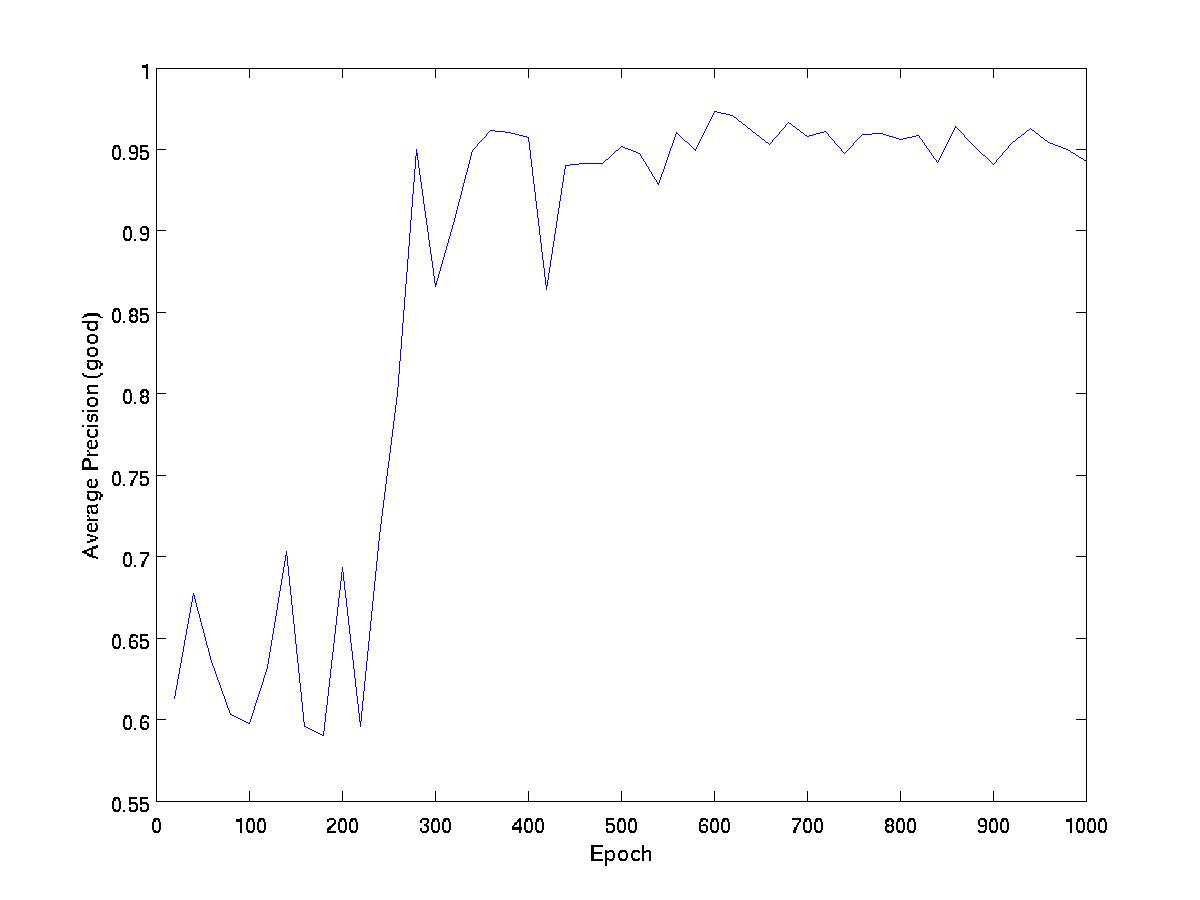
\includegraphics[width=0.96\columnwidth]{avg_prec}
\caption{\label{fig_graph} \small Training performance of the convolutional neural network over 1000 epochs. }
\end{figure}

\section{Discussion}

\subsection{Performance}
\label{sec_perf}

Its important to monitor the training of the neural network, because its very possible that the training database is insufficent.  Likely this is due to a lack of positive training samples.  For example, a boring game might not have a lot of ``cheering''.  Thus there are too few ``cheering'' samples with which to train the network.  Conversely, even in cases where there is demonstrable learning, the detector may produce ``false positives.''  This is likely due to a negative training set that is not complete.  Figure \ref{fig_results} hows some false positives produced by our clapping-fan detector.

\begin{figure}[bt]
\centering
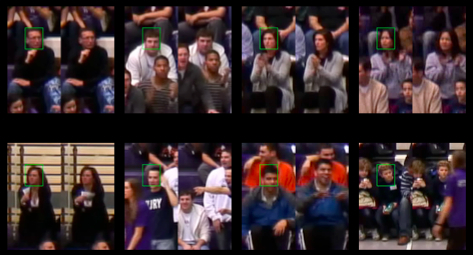
\includegraphics[width=0.96\columnwidth]{results}
\caption{\label{fig_results} \small On the top row, our clapping-fan detector predicts accurately (true positives).  On the bottom row, false positives are shown.  Left-to-right: a fan fanning themselves, a fan moves quickly out of view, a fan disagrees with a call, another fan walks in front of fan.   }
\end{figure}

With respect to processing time, the site-specific learning method we have demonstrated can begin right after video capture. Results could be ready a day after if not sooner.  Actually, much of the video processing like face detection and fidget generation can occur the moment the cameras dump footage.  Surprisingly, the labeling stage is not the most time consuming.  It took less than an hour for Amazon Mechanical Turk's team of anonymous workers to label the fan activity in 3000 fidgets.  The most time- and compute-intensive stage is the training the neural network.  On gpu-hardware, it can take several hours to train a convolutional neural network for 300 epochs using the architecture we described.

\subsection{Privacy}
\label{sec_privacy}

Legally speaking, there is no ``expectation of privacy'' at a public performance such as a sporting event.   And, in general, we are all gradually coming to terms with having little to no privacy from video surveillance, in many areas of their lives.  Still, game fans may not be too wild having their every move monitored and recorded at a game.  To remedy this, venues can choose to restrict viewing to only the resulting heatmap (Figure \ref{fig_fanheat}).  The heat-map stores the salient information anyway- indicating the presence, location and time of the activity of interest.  The heat-map essentially decouples the measurement of the fan's behavior from their identity.  The venue could go further, and, store only the result of the computations (the label predictions of the neural network) and delete the original crowd footage.  Technicians can always pull up the information later in heat-map form.

Although we did not do it in our experiment, it will also be possible to anonymize the face in the labeling task that we send to Amazon Mechanical Turk.  Google Maps has been doing this now for several years in their StreetView service and have published their approach \cite{streetview}.

\section{Future Work}

We want to explore not just other convolution neural network architectures, but also, other machine learning models, including those based on support vector machines.

The learning method, as proposed in this paper, starts from scratch for each event and each venue.  We believe that it should be possible to use instead, as a starting point, the trained algorithm from a previous event at the same venue, or possibly a different venue entirely.  Training samples from the new event are then used to incrementally refine an existing model.  Its possible this could speed up training by orders of magnitude.  This kind of ``active'' machine learning is also a possible future direction.

\section{Conclusion}

This paper described a machine learning-based method to detect specific kinds of fan activity in video footage.  We believe that this technique is a key component in a broader framework to understand audience engagement at sports events and other public performances.  Clubs and event venues can use these computer vision-based analytics to improve customer experience, retain fans, and ultimately, increase ticket revenue.

\section{Acknowledgements}
We would like to thank Will Freeman, Peggy Hackney, Chris Shell for useful discussions and pointers, and the Office of Naval Research (ONR N000140910076, N000140910789).


%-------------------------------------------------------------------------
{\tiny
\bibliographystyle{latex8}
\bibliography{vision}
}
\end{document}

